\documentclass[pdflatex,sn-basic,Numbered]{sn-jnl}

\usepackage{graphicx}%
\usepackage{multirow}%
\usepackage{amsmath,amssymb,amsfonts}%
\usepackage{amsthm}%
\usepackage{mathrsfs}%
\usepackage[title]{appendix}%
\usepackage{xcolor}%
\usepackage{textcomp}%
\usepackage{manyfoot}%
\usepackage{booktabs}%
\usepackage{longtable}%
\usepackage{array}%
\usepackage{ragged2e}%
\usepackage{pifont}%
\usepackage{float}%
\usepackage[spanish,es-tabla,es-noshorthands]{babel}%

\definecolor{gris}{gray}{0.35}
\newcommand{\si}{\ding{51}}
\newcommand{\no}{\textcolor{gris}{\textbf{--}}}
\newcommand{\pc}{\textbf{P}}
\newcommand{\nv}{\textsl{\footnotesize n/v}}
\newcommand{\nd}{\textsl{\footnotesize n/d}}

\theoremstyle{thmstyleone}
\newtheorem{theorem}{Theorem}
\newtheorem{proposition}[theorem]{Proposition}
\theoremstyle{thmstyletwo}
\newtheorem{example}{Example}
\newtheorem{remark}{Remark}
\theoremstyle{thmstylethree}
\newtheorem{definition}{Definition}

\raggedbottom

\begin{document}

\title[Privacidad y accesibilidad en sitios web universitarios]{Privacidad de datos personales en los sitios web de las mejores universidades del mundo: un contraste con las universidades del Ecuador}

\author*[1]{\fnm{Gleiston} \sur{Guerrero-Ulloa}}\email{gguerrero@uteq.edu.ec}
\author[2]{\fnm{Andrea} \sur{Zuñiga Paredes}}\email{andrear.zuniga@educacion.gob.ec}
\author[1]{\fnm{Efraín} \sur{Díaz-Macías}}\email{efraindiaz@uteq.edu.ec}

\affil*[1]{\orgdiv{Facultad de Ciencias de la Computación}, \orgname{Universidad Técnica Estatal de Quevedo}, \orgaddress{\street{Av. Quito Km 1.5 vía a Santo Domingo de los Tzáchilas S/N}, \city{Quevedo}, \postcode{120302}, \state{Los Ríos}, \country{Ecuador}}}
\affil[2]{\orgname{Ministerio de Educación de Ecuador}, \orgaddress{\city{Quito}, \country{Ecuador}}}

\abstract{La protección de datos personales en los sitios web universitarios es la cara visible de su gobernanza de la privacidad, pero apenas se ha medido en Ecuador. Este trabajo evalúa las 63 universidades y escuelas politécnicas ecuatorianas registradas en la SENESCYT y el CES, y las contrasta con las 63 mejores del mundo según los rankings QS 2026, THE 2026 y ARWU 2025. En cada sitio se examinaron el aviso de tratamiento, el marco legal citado, los derechos del titular y el responsable de datos, la seguridad y la accesibilidad, medida en vivo con un motor automático de conformidad WCAG. En gobernanza las brechas son amplias: en Ecuador el 61,9\,\% publica una política de privacidad, el 49,2\,\% cita la LOPDP y el 38,1\,\% designa un canal de contacto, frente al 92,1\,\%, 76,2\,\% y 85,7\,\% del referente mundial. En accesibilidad ninguna institución queda libre de fallos, pero su naturaleza difiere: el Ecuador incumple criterios de nivel básico (A) y el mundo solo los de excelencia (AAA). En las cookies, en cambio, no hay brecha: el 63,5\,\% de las IES ecuatorianas y el 68,3\,\% de las mejores del mundo cargan rastreo antes de todo consentimiento; así, el ``consentimiento de fachada'' es global y la contención europea no alcanza al visitante no comunitario. Accesibilidad y privacidad no se correlacionan. Las brechas propias del Ecuador están en la accesibilidad básica y en la gobernanza; se aporta una matriz reutilizable para el seguimiento del sector.}

\keywords{privacidad de datos, protecci\'on de datos personales, LOPDP, sitios web universitarios, cookies, accesibilidad web, educaci\'on superior, Ecuador}

\maketitle

\section{Introducci\'on}
El sitio web es hoy la puerta de entrada a la universidad: por él se postula, se consultan trámites, se accede a la matrícula y a los servicios, de modo que quedar fuera de esa puerta equivale a quedar fuera de la institución. Por eso la accesibilidad web ---que una persona con discapacidad visual, motriz o cognitiva pueda usar el portal en igualdad de condiciones--- no es un adorno técnico, sino una condición de acceso equitativo a la educación superior, y así lo reconocen las Pautas de Accesibilidad para el Contenido Web (WCAG) \citep{wcag21} y los marcos que las vuelven obligatorias, desde la \emph{European Accessibility Act} \citep{eaa2019} hasta la \emph{Americans with Disabilities Act} y la Sección 508 en Estados Unidos \citep{ada1990,section508}. Y sin embargo la evidencia reciente muestra que la promesa se cumple a medias incluso donde debería sobrar: las auditorías de portales universitarios encuentran barreras generalizadas, tanto en las mejores universidades del mundo evaluadas con WCAG 2.2 \citep{krittika2025accessibility} como en las europeas \citep{krejtz2025higher} o en los servicios públicos en línea \citep{aljedaani2025egovernment}, y en América Latina el rezago está documentado desde hace años \citep{campoverdemolina2023accessibility,acostavargas2020dataset}. La pregunta, entonces, no es si existen barreras, sino de qué tipo y qué tan hondas resultan en un sistema como el ecuatoriano.

La misma ventana que debe ser accesible es también el punto donde se juega la privacidad. Al abrir el portal, el visitante entrega datos al llenar un formulario de postulación, acepta o rechaza las \emph{cookies} que lo siguen entre páginas y busca ---cuando la institución ha hecho su tarea--- qué se hace con su información y cómo reclamar. En Ecuador esa dimensión llega tarde y despareja, algo esperable dada la juventud de la Ley Orgánica de Protección de Datos Personales (LOPDP), vigente desde 2021 y reglamentada apenas en 2023 \citep{lopdp2021,reglamentolopdp2023}. No es un problema solo local: en la última década buena parte del mundo adoptó regímenes inspirados en el modelo europeo \citep{gdpr2016}, y los estudios que midieron sus efectos coinciden en que la norma escrita y su cumplimiento real no marchan al mismo paso ---el Reglamento europeo multiplicó los avisos y las políticas, pero también los banners que empujan a aceptar y los textos más largos que legibles \citep{degeling2019value,kretschmer2021cookie}---, y en la educación superior no faltan universidades que retocaron sus políticas para aparentar conformidad antes que para garantizarla \citep{munot2025compliance}.

Accesibilidad y privacidad comparten así un mismo soporte ---el portal--- y una misma raíz ética: el respeto por quien lo usa. Cabe preguntarse si viajan juntas, es decir, si la universidad que se esfuerza por ser accesible cuida también los datos de su comunidad, o si cada compromiso sigue su propia suerte. Para responderlo con una escala reconocible, este trabajo somete al mismo examen a las 63 universidades mejor posicionadas del planeta ---tantas como las del censo nacional ecuatoriano--- y confronta ambos grupos en accesibilidad, uso de \emph{cookies}, aviso de tratamiento, seguridad y referencia al marco legal de cada jurisdicción, con auditorías automatizadas en vivo tanto de la conformidad WCAG como del comportamiento real de las \emph{cookies}. Elegir un referente de élite obedece a un razonamiento simple: si existe un estándar alto de práctica web, es ahí donde debería aparecer. El ejercicio no pretende medir a las universidades ecuatorianas más recientes ---la Universidad Pública de Santo Domingo de los Tsáchilas, creada en 2024, o la Universidad de Seguridad Ciudadana y Ciencias Policiales, todavía más nueva--- con la vara de Cambridge, sino aislar qué separa a unas de otras y qué resulta exigible bajo la ley. Conviene anticipar una advertencia que las páginas siguientes confirman: ni siquiera las mejores universidades del mundo ofrecen un modelo impecable, y esa imperfección es, por sí misma, un hallazgo aprovechable.

El resto del artículo se organiza como sigue. La Sección~\ref{sec:metodologia} describe cómo se construyó el conjunto de referencia por consenso de los tres rankings, qué dimensiones se evaluaron y cómo se adaptó el marco legal a cada jurisdicción, e incluye la auditoría en vivo del comportamiento de las \emph{cookies} y de la conformidad de accesibilidad. La Sección~\ref{sec:resultados} contrasta ambos grupos indicador por indicador, desglosa el conjunto mundial por regiones y presenta las mediciones en vivo del rastreo previo al consentimiento y de la conformidad WCAG. La Sección~\ref{sec:discusion} ordena las prioridades que se desprenden de la comparación, y la Sección~\ref{sec:conclusiones} sintetiza los hallazgos y propone una hoja de ruta. Por último, dos anexos reúnen, institución por institución, la evidencia que respalda cada cifra.

\section{Metodolog\'ia}\label{sec:metodologia}
La población de referencia surgió de condensar los tres rankings universitarios de mayor circulación en su edición más reciente: QS World University Rankings 2026, Times Higher Education 2026 y el Academic Ranking of World Universities (Shanghái) 2025 \citep{qs2026,the2026,arwu2025}. De cada uno se tomó el \emph{top} 75 y a cada universidad se le calculó el promedio de sus tres posiciones, computando como puesto 76 la ausencia del \emph{top} 75 de alguno. Por delante de ese promedio pesó el número de rankings en que la institución figuraba, así que las 46 presentes en los tres encabezan la lista y las 17 restantes salieron, por promedio, de entre las presentes en dos. El corte cayó en la Universidad de Queensland; la London School of Economics fue la primera en quedar fuera. Estados Unidos domina el grupo final con 24 instituciones, seguido de Europa continental (10), el Reino Unido (7), China (6) y una cola menor repartida entre Australia, Hong Kong, el resto de Asia y Canadá. La Figura~\ref{fig:mapa-paises} representa esa distribución geográfica sobre un mapa de calor.

\begin{figure}[!hbtp]
	\centering
	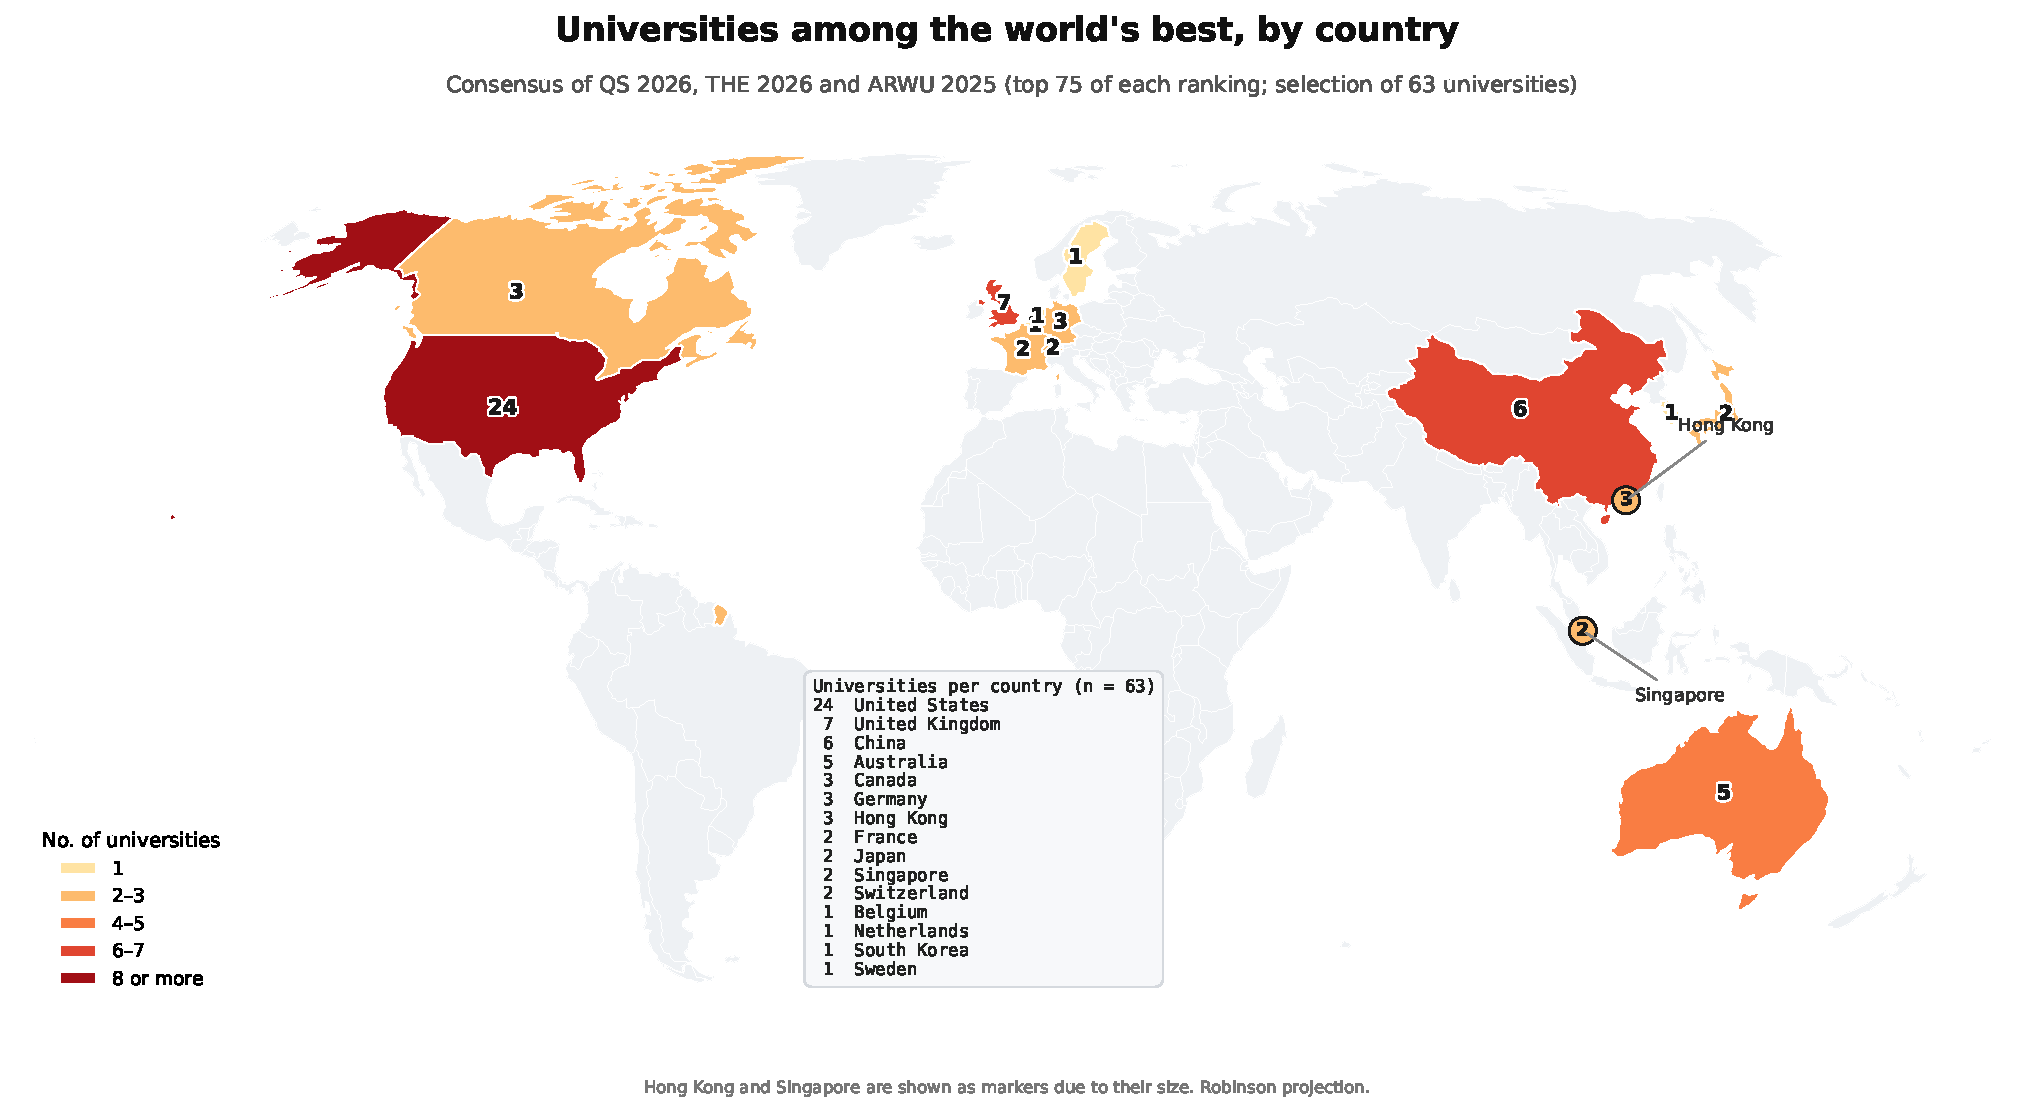
\includegraphics[width=\textwidth]{mapa_calor_paises.pdf}
	\caption{Distribución por país de las 63 universidades seleccionadas por consenso de QS 2026, THE 2026 y ARWU 2025. La intensidad del color indica el número de universidades por país; Hong Kong y Singapur se representan con marcadores por su reducido tamaño en el mapa.}
	\label{fig:mapa-paises}
\end{figure}

Cada sitio se revisó en agosto de 2026 con las cinco dimensiones del estudio ecuatoriano. Solo una exigió ajuste. Como la LOPDP rige únicamente en Ecuador \citep{lopdp2021,reglamentolopdp2023}, en el resto se comprobó si la institución cita el marco que le corresponde por jurisdicción: en Europa, el RGPD \citep{gdpr2016}, la ley británica de protección de datos \citep{ukdpa2018}, la normativa de \emph{ePrivacy} \citep{eprivacy2002} y la ley federal suiza \citep{fadp_ch}; en Estados Unidos, la CCPA \citep{ccpa2018}, la FERPA \citep{ferpa1974} y la HIPAA \citep{hipaa1996}; en China, la PIPL \citep{pipl2021}; en Japón, la APPI \citep{appi2003}; en Singapur, la PDPA \citep{pdpa2012}; en Corea del Sur, la PIPA \citep{pipa2011}; en Australia, la \emph{Privacy Act} \citep{privacyact1988}; en Canadá, la FIPPA o la ley de Quebec \citep{fippa_on,quebec_privacy}; y en Hong Kong, la PDPO \citep{pdpo_hk}. La Figura~\ref{fig:lineas-leyes} ordena cronológicamente estos marcos por su año de implementación.

\begin{figure}[!hbtp]
	\centering
	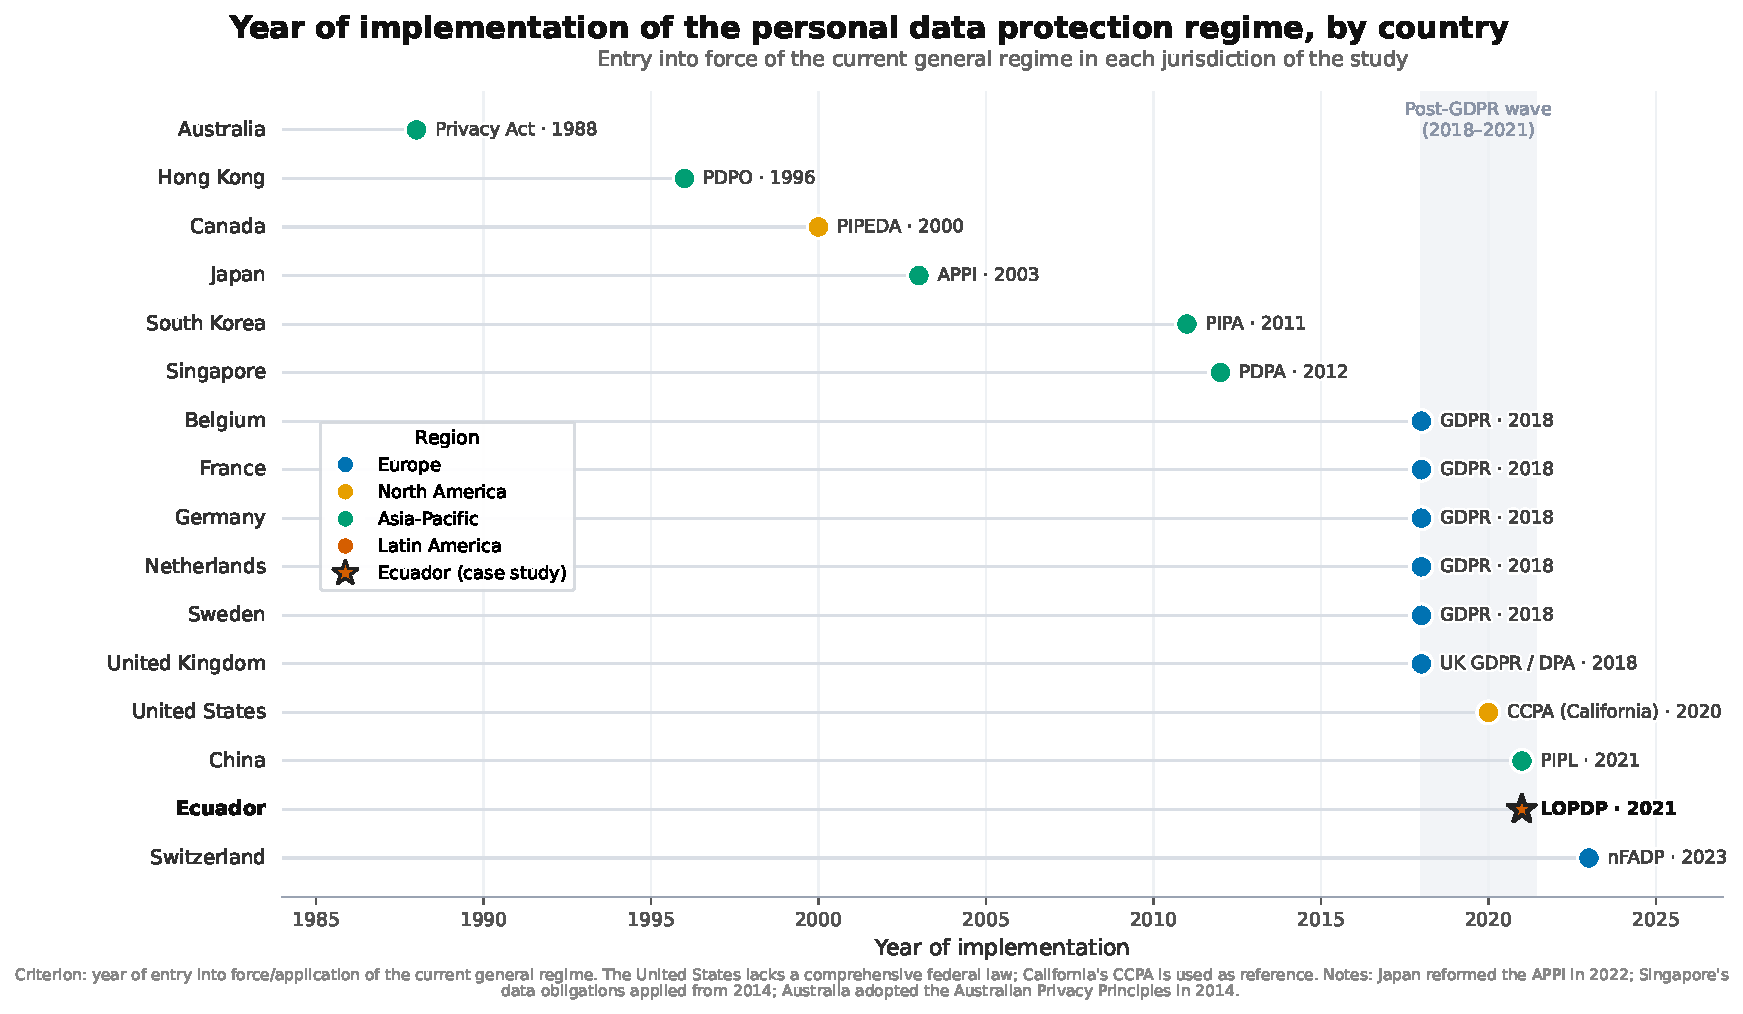
\includegraphics[width=\textwidth]{linea_tiempo_leyes.pdf}
	\caption{Año de implementación del régimen general de protección de datos personales en cada jurisdicción del estudio. Se toma la entrada en vigor o aplicación del régimen vigente; Estados Unidos carece de una ley federal integral, por lo que se usa la CCPA de California como referente. Ecuador se resalta como caso de estudio.}
	\label{fig:lineas-leyes}
\end{figure}

Esa cronología ayuda a situar el caso ecuatoriano. El arco va desde 1988, cuando Australia aprobó su \emph{Privacy Act}, hasta 2023, con la ley suiza revisada, y deja ver dos concentraciones: una difusión pausada a lo largo de los años 2000 y 2010, y un salto en 2018, cuando la aplicación del RGPD alineó en un mismo año a todo el bloque europeo y, de rebote, al Reino Unido. Ecuador (LOPDP, 2021) pertenece a la última oleada, junto con China (PIPL, 2021) y California (CCPA, 2020), de modo que su marco figura entre los más recientes del conjunto; esa juventud normativa ayuda a entender ---aunque no justifica--- que su traslación a la ventana web sea todavía incipiente, y sirve de telón de fondo para las diferencias que se examinan a continuación.

Las cuatro dimensiones restantes se conservaron intactas para que el contraste fuera legítimo, pero dos de ellas ---las \emph{cookies} y la accesibilidad--- se sometieron además a una auditoría automatizada \emph{en vivo}, porque el método documental no ejecuta JavaScript y subestima tanto los banners como las barreras que solo aparecen en la página renderizada. En agosto de 2026 se visitó cada uno de los 126 sitios con un navegador real ---Chromium controlado mediante Playwright--- desde una conexión en Ecuador, en una única pasada reproducible y con un guion de solo lectura. Antes de interactuar con ningún banner se registró el estado previo al consentimiento: el número y el nombre de las cookies, cuáles eran de rastreo (analítica y marketing), la firma de la plataforma de gestión del consentimiento (CMP) y la presencia de banner. En la misma carga se inyectó el motor axe-core 4.13 y se evaluó la conformidad con las Pautas de Accesibilidad para el Contenido Web \citep{wcag21}, asignando a cada incumplimiento su criterio, su principio ---perceptible, operable, comprensible o robusto--- y su nivel de conformidad (A, AA o AAA).

Conviene precisar el alcance de esta medición. Una herramienta automática demuestra el incumplimiento ---basta un fallo para romper un nivel--- pero no certifica la conformidad plena, pues buena parte de los criterios exige revisión humana y ninguna herramienta cubre por completo las pautas \citep{fischer2025coverage}; los resultados de axe cubren, por tanto, el subconjunto verificable por máquina, que en cada sitio se acompañó del número de comprobaciones que la propia herramienta marca para revisión manual. En las \emph{cookies}, medir desde un único punto de observación tiene una consecuencia buscada: los sitios sujetos al RGPD no muestran su banner ni bloquean el rastreo ante un visitante ajeno a la Unión Europea, de modo que lo observado es exactamente lo que experimenta un usuario ecuatoriano, no lo que vería un europeo.

\section{Resultados}\label{sec:resultados}
El Cuadro~\ref{tab:comp} pone frente a frente ambos conjuntos, indicador por indicador. El Cuadro~\ref{tab:reg} abre el grupo mundial por regiones, y los anexos recogen el detalle de cada institución: el Anexo~\ref{ap:mundo} (Cuadro~\ref{tab:mundo}) para las 63 del mundo y el Anexo~\ref{ap:ecuador} (Cuadro~\ref{tab:ecuador}) para las 63 del Ecuador.

\begin{table}[htbp]
	\centering
	\caption{Privacidad de datos en los sitios web: 63 mejores universidades del mundo frente a 63 IES del Ecuador.}
	\label{tab:comp}
	\small
	\begin{tabular}{@{}p{5.6cm}cccc@{}}
		\toprule
		\textbf{Indicador} & \textbf{Mundo} & \textbf{Mundo \%} & \textbf{Ecuador} & \textbf{Ecuador \%} \\
		\midrule
	Pol\'itica de privacidad / aviso de tratamiento & 58/63 & 92.1\% & 39/63 & 61.9\% \\
	Marco legal aplicable citado (LOPDP en Ecuador) & 48/63 & 76.2\% & 31/63 & 49.2\% \\
	Derechos del interesado enumerados & 47/63 & 74.6\% & 35/63 & 55.6\% \\
	Delegado (DPO) o contacto de datos & 54/63 & 85.7\% & 24/63 & 38.1\% \\
	Rastreo antes de consentir (en vivo) & 43/63 & 68.3\% & 40/63 & 63.5\% \\
	Gestor de consentimiento activo (CMP, en vivo) & 12/63 & 19.0\% & 14/63 & 22.2\% \\
	Accesibilidad / acci\'on afirmativa (declarada) & 47/63 & 74.6\% & 7/63 & 11.1\% \\
	Conformidad WCAG: alcanza nivel A (en vivo) & 25/63 & 39.7\% & 5/63 & 7.9\% \\
	Certificado TLS v\'alido & 63/63 & 100.0\% & 58/63 & 92.1\% \\
		\bottomrule
	\end{tabular}
	\par\vspace{2pt}
	\footnotesize\RaggedRight\textit{Nota:} ambos censos $n=63$. Las filas marcadas \emph{en vivo} provienen de la auditor\'ia en navegador real (agosto de 2026, axe-core 4.13) descrita en la metodolog\'ia; el resto, de la revisi\'on documental. ``Alcanza nivel A'' significa que el sitio no presenta fallos autom\'aticos de nivel A, el subconjunto verificable por m\'aquina de la conformidad WCAG.
\end{table}

\subsection{Aviso de tratamiento, marco legal y derechos}
La distancia mayor no aparece en los detalles técnicos, sino en los cimientos. Nueve de cada diez universidades del referente mundial publican una política de privacidad; en Ecuador lo hacen seis de cada diez. Si se exige además que esa política nombre el marco legal que la sustenta, el mundo baja al 76,2\,\% y Ecuador al 49,2\,\%. El desnivel se vuelve abismo en el punto que más importa a quien usa el sitio: saber a quién dirigirse. Un delegado de protección de datos o un canal específico consta en el 85,7\,\% de las mejores del mundo y en apenas el 38,1\,\% de las ecuatorianas, y la enumeración de los derechos del titular repite el sesgo, 74,6\,\% contra 55,6\,\%. Como estas cifras provienen de documentos que se leen sin renderizado alguno, el contraste es firme: a Ecuador no le falta tanto el papel como la profundidad jurídica de ese papel y una vía abierta para ejercer los derechos que enuncia.

Nada de esto convierte al referente en un dechado. Harvard, Michigan o Washington University in St.~Louis no enumeran derechos ni citan un marco en su aviso principal, y dos grandes universidades chinas, Fudan y Shanghai Jiao Tong, ni siquiera publican una política central en su portal institucional. Que instituciones de ese calibre arrastren semejantes vacíos recuerda que el prestigio académico no asegura el cuidado de los datos, y confirma que la conformidad puede ser más apariencia que sustancia \citep{munot2025compliance}.

\subsection{Uso de \emph{cookies}}
El método estático no veía los banners ni las cookies que inyecta el JavaScript, así que esta dimensión se comprobó \emph{en vivo}, visitando cada sitio en un navegador real y registrando, antes de cualquier consentimiento, qué cookies se depositaban, qué plataforma de gestión del consentimiento (CMP) cargaba y si aparecía un banner. La Figura~\ref{fig:cookies-live} resume el contraste y desmiente la lectura ingenua de que un banner escaso significa poco rastreo.

\begin{figure}[H]
	\centering
	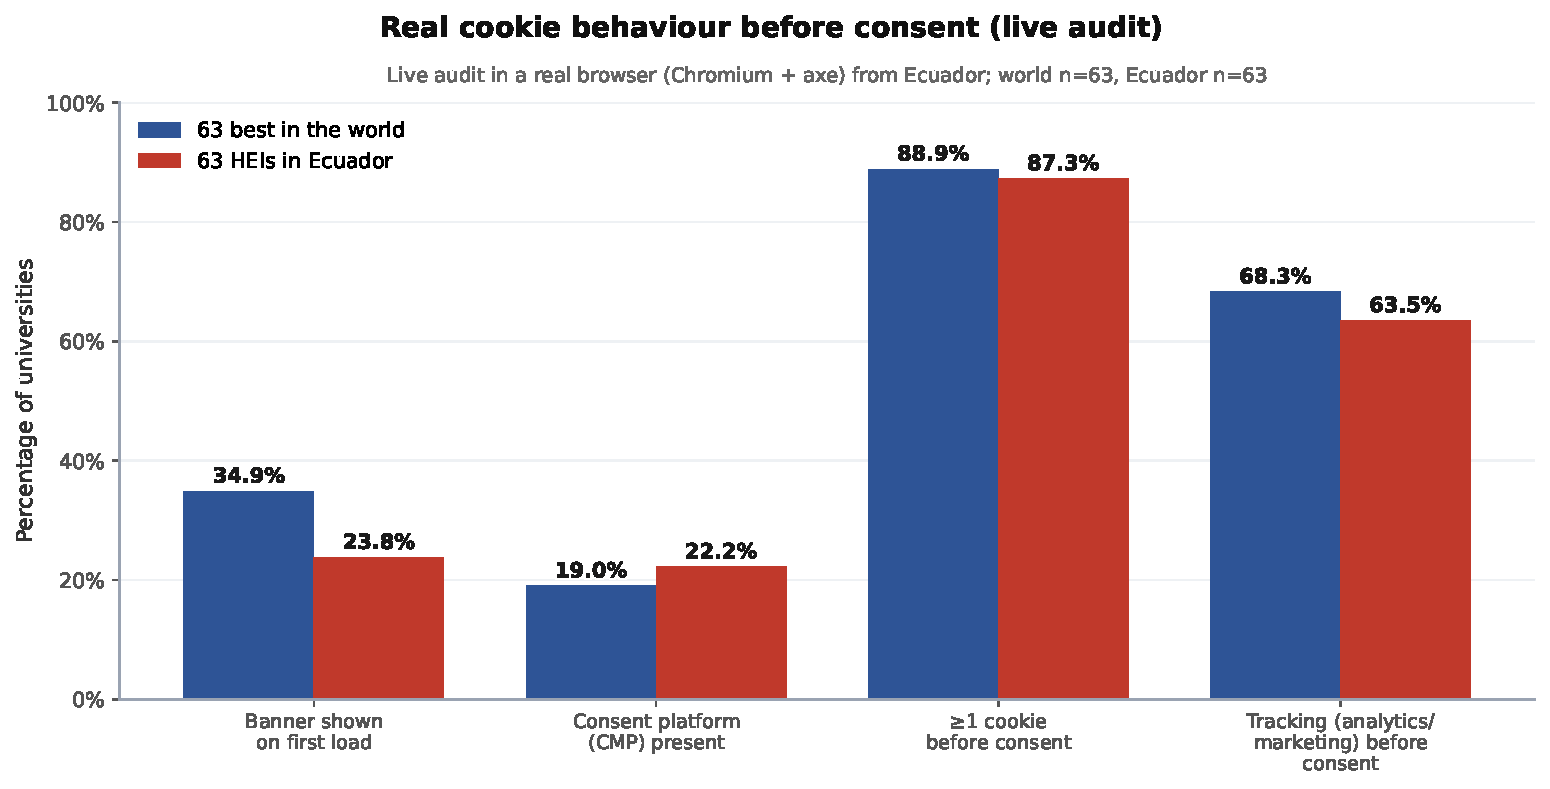
\includegraphics[width=\textwidth]{fig_cookies_live.pdf}
	\caption{Verificación en vivo del comportamiento de \emph{cookies} antes del consentimiento: 63 mejores universidades del mundo frente a las 63 IES del Ecuador (mundo $n=63$; Ecuador $n=63$). En cada sitio se leyó el estado previo a cualquier interacción con el banner.}
	\label{fig:cookies-live}
\end{figure}

El banner visible es minoritario en ambos lados (34,9\,\% en el mundo, 23,8\,\% en Ecuador), pero esa foto instantánea engaña, porque muchos sitios europeos solo lo muestran a visitantes de la Unión Europea y esta auditoría se realizó desde Ecuador. Lo revelador está en las cookies que se colocan \emph{sin} mediar consentimiento, y ahí no hay brecha: en Ecuador el 87,3\,\% deposita al menos una y el 63,5\,\% carga cookies de rastreo ---analítica o marketing: Google Analytics y Ads, el píxel de Meta, TikTok, Microsoft Clarity o Hotjar---; en las mejores del mundo esas cifras son, si acaso, algo mayores: 88,9\,\% y 68,3\,\%. Vista desde el navegador de un usuario ecuatoriano, la élite mundial rastrea antes del consentimiento tanto como las universidades del país, o un poco más.

Ese resultado obliga a corregir una intuición cómoda. La contención que suele atribuirse a las universidades sujetas al RGPD no protege a quien las visita desde fuera de la Unión Europea: ante un usuario ecuatoriano no aparece el banner ni se bloquea el rastreo, que se dispara igual. El ``consentimiento de fachada'' ---interfaces que inducen a aceptar y disimulan el rechazo, o gestores de \emph{cookies} que en realidad no bloquean--- no es entonces un defecto local sino un fenómeno global, y la presencia de una CMP, algo más común en Ecuador (22,2\,\%) que en el mundo (19,0\,\%), no altera el desenlace. Es justo lo que la literatura de medición describió tras el RGPD, cuando se multiplicaron los avisos sin que mejorara el tratamiento: la mera presencia de un banner no garantiza un consentimiento válido \citep{degeling2019value,kretschmer2021cookie,nouwens2020dark,gray2021dark,habib2022okay}.

\subsection{Acci\'on afirmativa, inclusi\'on y seguridad}
La otra grieta honda es la accesibilidad, tomada aquí como vehículo de inclusión. Tres de cada cuatro universidades de élite ofrecen una declaración o herramientas de accesibilidad; en Ecuador lo hace una de cada nueve. Detrás de esa diferencia pesan obligaciones legales concretas, como la \emph{Americans with Disabilities Act} \citep{ada1990} y la Sección 508 de la \emph{Rehabilitation Act} \citep{section508} en Estados Unidos o la \emph{European Accessibility Act} \citep{eaa2019} en la Unión Europea, y del lado ecuatoriano una práctica casi inexistente en los portales, rezago que la investigación regional documenta desde hace años \citep{campoverdemolina2023accessibility,acostavargas2020dataset}. En el cifrado de las comunicaciones la historia es más benévola: el HTTPS válido cubre al 100\,\% del grupo mundial y al 92,1\,\% del ecuatoriano, donde cinco instituciones cargan con certificados defectuosos.

\begin{table}[!htbp]
	\centering
	\caption{Conjunto mundial por regi\'on: pol\'itica de privacidad, marco legal citado, DPO y accesibilidad (IES que cumplen sobre el total regional).}
	\label{tab:reg}
	\small
	\begin{tabular}{@{}lccccc@{}}
		\toprule
		\textbf{Regi\'on} & \textbf{n} & \textbf{Privacidad} & \textbf{Marco legal} & \textbf{DPO} & \textbf{Accesib.} \\
		\midrule
	EE.UU. & 24 & 24 & 18 & 23 & 22 \\
	Reino Unido & 7 & 6 & 4 & 5 & 7 \\
	Europa continental & 10 & 10 & 9 & 10 & 8 \\
	China & 6 & 2 & 2 & 3 & 0 \\
	Hong Kong & 3 & 3 & 3 & 2 & 3 \\
	Asia (otros) & 5 & 5 & 4 & 4 & 0 \\
	Australia & 5 & 5 & 5 & 4 & 4 \\
	Canadá & 3 & 3 & 3 & 3 & 3 \\
		\bottomrule
	\end{tabular}
\end{table}

El desglose por regiones desarma la idea de un ``mundo desarrollado'' homogéneo. Europa continental encabeza la referencia al marco legal, con nueve de sus diez universidades citando el RGPD y su transposición nacional; Estados Unidos manda en accesibilidad, con 22 de 24 portales, empujado por la ADA; y las tres casas de Hong Kong cumplen sin fisuras al amparo de la PDPO. China es la excepción del grupo: solo dos de sus seis universidades nombran un marco legal y ninguna publica declaración de accesibilidad. La moraleja es que ocupar la cima de la investigación mundial y cuidar la privacidad en la web son asuntos distintos, que no siempre viajan juntos.

\subsection{Conformidad WCAG medida}
La accesibilidad declarada del Cuadro~\ref{tab:comp} solo dice si la institución promete inclusión; para saber si la cumple se auditó cada portal con axe-core, contrastando su código contra los criterios de las WCAG. El Cuadro~\ref{tab:wcag} resume el resultado y la Figura~\ref{fig:wcag-niveles} muestra su rasgo más ilustrativo.

\begin{table}[htbp]
	\centering
	\caption{Conformidad WCAG medida en vivo (axe-core): 63 mejores del mundo frente a 63 IES del Ecuador. Porcentaje de sitios salvo indicaci\'on.}
	\label{tab:wcag}
	\small
	\begin{tabular}{@{}p{8.4cm}cc@{}}
		\toprule
		\textbf{Indicador (auditor\'ia en vivo)} & \textbf{Mundo} & \textbf{Ecuador} \\
		\midrule
	Violaciones WCAG por sitio (mediana) & 2 & 4 \\
	Sitios sin ning\'un fallo autom\'atico & 9.5\% & 0.0\% \\
	Sitios que alcanzan el nivel A & 39.7\% & 7.9\% \\
	Enlaces sin nombre accesible (2.4.4, nivel A) & 23.8\% & 81.0\% \\
	Contraste insuficiente (1.4.3, nivel AA) & 25.4\% & 79.4\% \\
	Im\'agenes sin alternativa textual (1.1.1, nivel A) & 15.9\% & 30.2\% \\
	Nivel donde se concentran los fallos & AAA & A \\
		\bottomrule
	\end{tabular}
\end{table}

\begin{figure}[H]
	\centering
	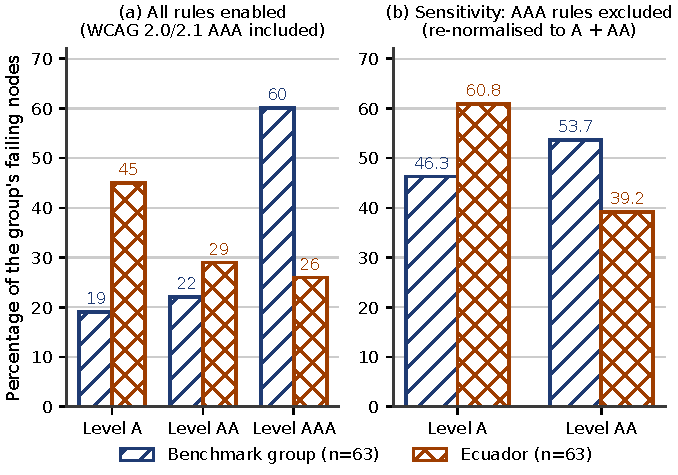
\includegraphics[width=\textwidth]{fig_wcag_niveles.pdf}
	\caption{Distribuci\'on de los nodos con fallo WCAG por nivel de conformidad (porcentaje del total de cada grupo; axe-core, agosto de 2026). El Ecuador concentra sus fallos en el nivel A ---el b\'asico---, mientras que las mejores del mundo lo hacen en el nivel AAA ---el de excelencia---.}
	\label{fig:wcag-niveles}
\end{figure}

Los números desmienten cualquier autocomplacencia por ambos lados: ninguna universidad ecuatoriana ---y solo el 9,5\,\% de las mejores del mundo--- pasa la auditoría sin un solo fallo automático, y la mediana de violaciones por sitio es de cuatro en Ecuador frente a dos en el mundo. Pero la diferencia decisiva no está en la cantidad, sino en la gravedad. En el referente mundial, el 60\,\% de los nodos con fallo pertenece al nivel AAA ---el de excelencia, sobre todo el contraste realzado---, y apenas el 19\,\% cae en el nivel A; en Ecuador la proporción se invierte y el 45\,\% de los fallos afecta a ese nivel A, el más básico. Dicho de otro modo, el mundo tropieza persiguiendo la excelencia y Ecuador tropieza en el umbral. El caso más elocuente es el criterio 2.4.4, que pide que cada enlace tenga un texto que un lector de pantalla pueda anunciar: lo incumple el 81,0\,\% de los sitios ecuatorianos frente al 23,8\,\% del mundo. El principio más golpeado en ambos grupos es el perceptible, por el contraste de color, pero en Ecuador se le suma un déficit operable ---enlaces y controles--- que en el referente es marginal; son, por lo demás, los mismos tipos de error que dominan las auditorías WCAG de otros portales públicos \citep{iniesto2025service}.

Reunidas las dos auditorías en vivo aflora un hallazgo que trasciende al ranking: la calidad de la accesibilidad y el respeto por la privacidad no van de la mano. Entre las 126 universidades, la correlación entre el volumen de fallos de accesibilidad y la cantidad de \emph{cookies} de rastreo es prácticamente nula (Spearman $\rho=0{,}04$). Cuidar una cosa no predice cuidar la otra: en Ecuador, una de cada tres instituciones limita el rastreo pero falla la accesibilidad básica, y apenas un 3\,\% logra ambas; en el mundo, un 30\,\% es accesible en el nivel A y aun así rastrea sin permiso. Son, por tanto, dos compromisos éticos independientes ---accesibilidad e intimidad---, cada uno con su propia palanca legal y su propia inercia, y ninguna universidad, del país o del planeta, los ha resuelto a la vez.

\section{Discusi\'on}\label{sec:discusion}
La comparación ordena las prioridades del sistema ecuatoriano. Lo apremiante no es la infraestructura, con un HTTPS ya casi generalizado, ni el banner de \emph{cookies}, indicador escurridizo y de calidad dudosa hasta entre los líderes. Lo apremiante es la gobernanza: una política anclada en la ley, unos derechos redactados con claridad y, por encima de todo, un responsable de datos al que se pueda escribir y un portal que cualquiera pueda usar. Que las universidades de élite cumplan estos puntos con tanta frecuencia no es mérito espontáneo, sino respuesta a leyes que los imponen, desde la obligación del RGPD de nombrar un delegado hasta los mandatos de accesibilidad de la ADA. La LOPDP y su reglamento encierran exigencias equivalentes, todavía poco visibles en la ventana pública de las instituciones.

El referente, aun así, aconseja no idealizar. Contar con una política no prueba un buen tratamiento; los banners de las universidades más reputadas incumplen a menudo las condiciones de un consentimiento libre \citep{nouwens2020dark,gray2021dark}; y hasta nombres de primerísima fila muestran huecos difíciles de justificar. La meta sensata para Ecuador no es copiar la fachada de esas instituciones, sino alcanzar lo que su fachada a veces esconde y que la ley ya reclama: un tratamiento respetuoso de los datos de su comunidad.

El dato en vivo añade un matiz que corrige la lectura fácil. En el papel Ecuador va por detrás, pero en el comportamiento real de las \emph{cookies} no existe tal brecha: sus universidades rastrean al usuario antes de pedirle permiso casi tanto como las mejores del mundo (63,5\,\% frente a 68,3\,\%), y estas, vistas desde fuera de la Unión Europea, no se comportan mejor. El ``consentimiento de fachada'' es un problema compartido, no una singularidad ecuatoriana; y como la protección del RGPD se detiene en la frontera comunitaria, el estudiante que consulta desde Ecuador el portal de una universidad europea queda tan expuesto como en el de su propia institución. La lección para Ecuador no es, por tanto, que rastree más que nadie, sino que la solución no vendrá de imitar una contención que el referente solo aplica de puertas adentro.

\section{Conclusiones}\label{sec:conclusiones}
Medido contra las 63 mejores universidades del mundo, el sistema ecuatoriano exhibe brechas anchas justo donde más se juega la confianza de las personas: políticas ancladas en la ley (61,9\,\% frente a 92,1\,\%) y delegado o canal de protección de datos (38,1\,\% frente a 85,7\,\%). A ellas se suma la accesibilidad, donde la auditoría en vivo revela que ninguna institución queda libre de fallos, pero que Ecuador incumple criterios de nivel básico ---el 81\,\% de sus sitios tiene enlaces sin nombre accesible--- mientras el mundo solo tropieza en los de excelencia. Ese es el orden en que conviene actuar. La verificación en vivo, en cambio, matiza el frente de las \emph{cookies}: dos de cada tres IES ecuatorianas rastrean al usuario antes de pedirle permiso, pero las mejores del mundo lo hacen en igual medida ante un visitante no europeo, de modo que el problema es global y no una falla propia del país. Publicar una política que invoque de forma expresa la LOPDP y su reglamento, poner nombre y correo a un responsable de datos, hacer accesibles los portales según las pautas WCAG \citep{wcag21} ---empezando por lo básico--- y exigir a los gestores de \emph{cookies} que de verdad bloqueen bastaría para cerrar la mayor parte de la distancia. Persiste un reto que Ecuador comparte con Cambridge o el MIT y que ninguna estadística de portada resuelve: que lo prometido en la página se cumpla de verdad en el tratamiento.

\begin{appendices}
\section{Anexos}
Los anexos reúnen la evidencia institución por institución en que se apoyan las cifras de este trabajo, para que el conteo pueda rehacerse y los casos individuales auditarse. El Anexo~\ref{ap:mundo} recoge las 63 universidades del mundo (Cuadro~\ref{tab:mundo}) y el Anexo~\ref{ap:ecuador} las 63 instituciones ecuatorianas (Cuadro~\ref{tab:ecuador}). En ambos, cada fila es un sitio web oficial y cada columna una de las dimensiones evaluadas, con la misma leyenda de marcadores; las columnas no coinciden por completo entre uno y otro porque el marco legal se adaptó a cada jurisdicción y porque la transparencia (LOTAIP) solo aplica al caso ecuatoriano. Las direcciones exactas y las fechas de consulta constan en las matrices de datos que acompañan a este trabajo.

\section{Matriz de las 63 mejores universidades del mundo}
\label{ap:mundo}
Leyenda: \si~cumple; \no~ausente o no cumple; \textbf{P}~parcial (\'ambito acotado o marco gen\'erico); \nd~no detectable (contenido din\'amico). Rankings: QS 2026, THE 2026 y ARWU 2025 (puesto; ``--'' indica fuera del \emph{top} 75 de ese ranking). Pa\'is en c\'odigo ISO. Columnas: Pol.\ (pol\'itica de privacidad), Marco (marco legal citado), Der.\ (derechos), DPO, Cook.\ (pol\'itica de \emph{cookies}), Acc.\ (accesibilidad).

\footnotesize
\begin{longtable}{@{}r l c c c c c c c c c c@{}}
	\caption{Matriz de privacidad de datos de las 63 mejores universidades del mundo.}\label{tab:mundo}\\
	\toprule
	\textbf{\#} & \textbf{Sigla} & \textbf{P} & \textbf{QS} & \textbf{THE} & \textbf{ARWU} & \textbf{Pol.} & \textbf{Marco} & \textbf{Der.} & \textbf{DPO} & \textbf{Cook.} & \textbf{Acc.} \\
	\midrule
	\endfirsthead
	\multicolumn{12}{c}{\textit{(Cuadro~\ref{tab:mundo}, continuaci\'on)}}\\
	\toprule
	\textbf{\#} & \textbf{Sigla} & \textbf{P} & \textbf{QS} & \textbf{THE} & \textbf{ARWU} & \textbf{Pol.} & \textbf{Marco} & \textbf{Der.} & \textbf{DPO} & \textbf{Cook.} & \textbf{Acc.} \\
	\midrule
	\endhead
	\midrule
	\multicolumn{12}{r}{\textit{Contin\'ua en la siguiente p\'agina}}\\
	\endfoot
	\bottomrule
	\endlastfoot
	1 & MIT & US & 1 & 2 & 3 & \si & \si & \si & \si & \no & \si \\
	2 & Stanford & US & 3 & 5 & 2 & \si & \si & \si & \si & \si & \si \\
	3 & Harvard & US & 5 & 5 & 1 & \si & \si & \no & \no & \no & \si \\
	4 & Oxford & UK & 4 & 1 & 6 & \si & \si & \si & \si & \si & \si \\
	5 & Cambridge & UK & 6 & 3 & 4 & \no & \pc & \no & \no & \si & \si \\
	6 & Caltech & US & 10 & 7 & 9 & \si & \si & \no & \si & \no & \si \\
	7 & UC Berkeley & US & 17 & 9 & 5 & \si & \si & \no & \si & \no & \si \\
	8 & Princeton & US & 25 & 3 & 7 & \si & \si & \si & \si & \no & \si \\
	9 & Imperial & UK & 2 & 8 & 26 & \si & \si & \pc & \no & \si & \si \\
	10 & U Chicago & US & 13 & 15 & 10 & \si & \pc & \si & \si & \no & \no \\
	11 & ETH Zurich & CH & 7 & 11 & 22 & \si & \si & \si & \si & \no & \si \\
	12 & Yale & US & 21 & 10 & 11 & \si & \si & \pc & \si & \no & \si \\
	13 & UPenn & US & 15 & 14 & 14 & \si & \pc & \si & \si & \no & \si \\
	14 & UCL & UK & 9 & 22 & 14 & \si & \pc & \si & \si & \si & \si \\
	15 & Cornell & US & 16 & 18 & 12 & \si & \pc & \si & \si & \no & \si \\
	16 & Tsinghua & CN & 17 & 12 & 18 & \si & \si & \si & \si & \no & \no \\
	17 & Peking & CN & 14 & 13 & 23 & \pc & \pc & \no & \no & \no & \no \\
	18 & Johns Hopkins & US & 24 & 16 & 19 & \si & \si & \si & \si & \no & \si \\
	19 & Columbia & US & 38 & 20 & 8 & \si & \si & \si & \si & \si & \si \\
	20 & Toronto & CA & 29 & 21 & 25 & \si & \si & \si & \si & \no & \si \\
	21 & UCLA & US & 46 & 18 & 16 & \si & \si & \si & \si & \no & \si \\
	22 & NUS & SG & 8 & 17 & 56 & \si & \si & \si & \si & \no & \no \\
	23 & U Tokyo & JP & 36 & 26 & 31 & \si & \si & \si & \no & \no & \no \\
	24 & TUM & DE & 22 & 27 & 45 & \si & \si & \si & \si & \no & \no \\
	25 & Melbourne & AU & 19 & 37 & 38 & \si & \si & \si & \si & \no & \no \\
	26 & Edinburgh & UK & 34 & 29 & 37 & \si & \si & \si & \si & \no & \si \\
	27 & EPFL & CH & 22 & 35 & 44 & \si & \si & \si & \si & \no & \si \\
	28 & Michigan & US & 45 & 23 & 33 & \si & \no & \no & \si & \no & \no \\
	29 & Northwestern & US & 42 & 30 & 31 & \si & \pc & \si & \si & \si & \si \\
	30 & Fudan & CN & 30 & 36 & 41 & \no & \no & \no & \no & \no & \no \\
	31 & PSL & FR & 28 & 48 & 34 & \si & \si & \si & \si & \no & \no \\
	32 & HKU & HK & 11 & 33 & 67 & \si & \si & \si & \si & \no & \si \\
	33 & Zhejiang & CN & 49 & 39 & 24 & \si & \pc & \si & \si & \no & \no \\
	34 & NYU & US & 55 & 31 & 28 & \si & \si & \si & \si & \no & \si \\
	35 & SJTU & CN & 47 & 40 & 30 & \no & \no & \no & \no & \no & \no \\
	36 & KCL & UK & 31 & 38 & 61 & \si & \pc & \si & \si & \si & \si \\
	37 & UCSD & US & 66 & 47 & 20 & \si & \si & \si & \si & \no & \si \\
	38 & LMU & DE & 58 & 34 & 42 & \si & \si & \si & \si & \no & \si \\
	39 & Duke & US & 62 & 28 & 46 & \si & \si & \si & \si & \no & \si \\
	40 & Manchester & UK & 35 & 56 & 46 & \si & \si & \pc & \si & \no & \si \\
	41 & UBC & CA & 40 & 45 & 53 & \si & \si & \pc & \si & \no & \si \\
	42 & Sydney & AU & 25 & 53 & 72 & \si & \si & \si & \si & \no & \si \\
	43 & Paris-Saclay & FR & 70 & 68 & 13 & \si & \si & \si & \si & \si & \si \\
	44 & Kyoto & JP & 57 & 61 & 46 & \si & \pc & \si & \si & \no & \no \\
	45 & Illinois & US & 70 & 41 & 53 & \si & \si & \si & \si & \no & \si \\
	46 & UT Austin & US & 68 & 50 & 49 & \si & \si & \si & \si & \no & \si \\
	47 & UW & US & -- & 25 & 17 & \si & \si & \si & \si & \no & \si \\
	48 & NTU & SG & 12 & 31 & -- & \si & \si & \si & \si & \no & \no \\
	49 & McGill & CA & 27 & 41 & -- & \si & \si & \si & \si & \si & \si \\
	50 & CUHK & HK & 32 & 41 & -- & \si & \si & \si & \no & \no & \si \\
	51 & CMU & US & 52 & 24 & -- & \si & \si & \si & \si & \no & \si \\
	52 & Wisconsin & US & -- & 53 & 36 & \si & \si & \no & \si & \si & \si \\
	53 & USTC & CN & -- & 51 & 40 & \pc & \si & \si & \si & \no & \no \\
	54 & WUSTL & US & -- & 67 & 26 & \si & \no & \no & \si & \no & \si \\
	55 & Monash & AU & 36 & 58 & -- & \si & \si & \no & \no & \no & \si \\
	56 & SNU & KR & 38 & 58 & -- & \si & \si & \si & \si & \no & \no \\
	57 & Heidelberg & DE & -- & 49 & 51 & \si & \si & \si & \si & \no & \si \\
	58 & HKUST & HK & 44 & 58 & -- & \si & \si & \si & \si & \no & \si \\
	59 & Karolinska & SE & -- & 53 & 50 & \si & \pc & \si & \si & \si & \si \\
	60 & TU Delft & NL & 47 & 57 & -- & \si & \si & \si & \si & \si & \si \\
	61 & ANU & AU & 32 & 73 & -- & \si & \si & \pc & \si & \no & \si \\
	62 & KU Leuven & BE & 60 & 46 & -- & \si & \si & \si & \si & \si & \si \\
	63 & Queensland & AU & 42 & -- & 65 & \si & \si & \si & \si & \no & \si \\
\end{longtable}
\normalsize

\section{Matriz de las 63 IES del Ecuador (SENESCYT/CES)}
\label{ap:ecuador}
Se reproduce, para facilitar el cotejo, la matriz del censo ecuatoriano. Leyenda: \si~cumple; \no~ausente o no cumple; \textbf{P}~parcial (ámbito acotado, por ejemplo solo posgrado, admisión o aplicación móvil); \nv~no verificable por el método (sitio bloqueado o documento no legible por máquina); \nd~no detectable (contenido dinámico). Tipo: P (pública), C (cofinanciada), A (autofinanciada). Columnas: Pol.\ (política de privacidad), LOPDP (mención expresa de la ley), Der.\ (derechos), DPO, Cook.\ (banner de \emph{cookies}), Incl.\ (accesibilidad/inclusión), Transp.\ (transparencia/LOTAIP).

\footnotesize
\begin{longtable}{@{}r l c c c c c c c c@{}}
	\caption{Matriz de privacidad de datos de las 63 IES del Ecuador.}\label{tab:ecuador}\\
	\toprule
	\textbf{\#} & \textbf{Sigla} & \textbf{Tipo} & \textbf{Pol.} & \textbf{LOPDP} & \textbf{Der.} & \textbf{DPO} & \textbf{Cook.} & \textbf{Incl.} & \textbf{Transp.} \\
	\midrule
	\endfirsthead
	\multicolumn{10}{c}{\textit{(Cuadro~\ref{tab:ecuador}, continuación)}}\\
	\toprule
	\textbf{\#} & \textbf{Sigla} & \textbf{Tipo} & \textbf{Pol.} & \textbf{LOPDP} & \textbf{Der.} & \textbf{DPO} & \textbf{Cook.} & \textbf{Incl.} & \textbf{Transp.} \\
	\midrule
	\endhead
	\midrule
	\multicolumn{10}{r}{\textit{Continúa en la siguiente página}}\\
	\endfoot
	\bottomrule
	\endlastfoot
	1 & EPN & P & \si & \si & \si & \no & \nd & \no & \si \\
	2 & ESPOL & P & \si & \si & \si & \si & \nd & \no & \si \\
	3 & ESPOCH & P & \no & \no & \no & \no & \nd & \no & \si \\
	4 & ESPAM MFL & P & \no & \no & \no & \no & \nd & \no & \si \\
	5 & ESPE & P & \si & \si & \si & \si & \nd & \si & \si \\
	6 & UCE & P & \nv & \no & \no & \no & \nd & \no & \si \\
	7 & UCuenca & P & \si & \si & \si & \no & \si & \no & \si \\
	8 & UG & P & \si & \si & \si & \si & \nd & \no & \si \\
	9 & UNL & P & \no & \no & \no & \no & \nd & \no & \si \\
	10 & UAE & P & \no & \no & \no & \no & \nd & \no & \si \\
	11 & UTA & P & \si & \nv & \nv & \nv & \nd & \nv & \si \\
	12 & UTB & P & \si & \si & \si & \si & \nd & \no & \si \\
	13 & UTC & P & \si & \no & \no & \no & \nd & \no & \nd \\
	14 & UTMACH & P & \si & \si & \si & \si & \nd & \no & \si \\
	15 & UTM & P & \no & \no & \no & \no & \nd & \no & \si \\
	16 & UTN & P & \pc & \si & \si & \no & \nd & \no & \si \\
	17 & UTEQ & P & \pc & \si & \no & \no & \nd & \no & \si \\
	18 & UTELVT & P & \no & \no & \no & \no & \nd & \no & \si \\
	19 & UEB & P & \si & \nv & \nv & \nv & \nd & \si & \si \\
	20 & UNESUM & P & \pc & \nv & \no & \no & \nd & \no & \si \\
	21 & UNEMI & P & \si & \si & \si & \no & \nd & \no & \si \\
	22 & UEA & P & \si & \no & \si & \no & \nd & \no & \si \\
	23 & UPSE & P & \pc & \si & \si & \si & \nd & \pc & \si \\
	24 & ULEAM & P & \no & \no & \no & \no & \nd & \no & \si \\
	25 & UNACH & P & \si & \si & \si & \si & \nd & \si & \si \\
	26 & UNAE & P & \no & \no & \no & \no & \nd & \no & \si \\
	27 & UPEC & P & \no & \pc & \no & \no & \nd & \no & \si \\
	28 & Yachay Tech & P & \no & \no & \no & \no & \nd & \no & \si \\
	29 & Ikiam & P & \si & \si & \si & \si & \nd & \no & \si \\
	30 & UArtes & P & \si & \si & \si & \si & \nd & \no & \si \\
	31 & Amawtay Wasi & P & \no & \no & \no & \no & \nd & \no & \si \\
	32 & USECIPOL & P & \pc & \no & \no & \no & \nd & \no & \si \\
	33 & IAEN & P & \si & \si & \si & \no & \si & \si & \si \\
	34 & UASB & P & \si & \si & \si & \si & \nd & \no & \si \\
	35 & FLACSO & P & \no & \no & \no & \no & \nd & \no & \si \\
	36 & PUCE & C & \si & \si & \si & \si & \nd & \no & \si \\
	37 & UCSG & C & \si & \si & \si & \si & \si & \no & \si \\
	38 & UCACUE & C & \si & \si & \si & \si & \nd & \si & \si \\
	39 & ULVR & C & \no & \no & \no & \no & \nd & \no & \si \\
	40 & UTPL & C & \si & \si & \si & \si & \nd & \no & \nd \\
	41 & UTE & C & \si & \no & \no & \no & \nd & \si & \nd \\
	42 & UDA & C & \no & \no & \no & \no & \nd & \no & \si \\
	43 & UPS & C & \si & \si & \si & \no & \nd & \no & \si \\
	44 & UISEK & A & \si & \no & \si & \no & \nd & \no & \no \\
	45 & UEES & A & \si & \si & \si & \si & \nd & \no & \no \\
	46 & USFQ & A & \si & \si & \si & \si & \nd & \no & \no \\
	47 & UDLA & A & \si & \si & \si & \si & \nd & \no & \no \\
	48 & UIDE & A & \si & \si & \si & \si & \nd & \no & \si \\
	49 & UNIANDES & A & \si & \no & \si & \no & \nd & \no & \no \\
	50 & UPACÍFICO & A & \nv & \no & \no & \no & \nd & \no & \no \\
	51 & UTI & A & \si & \no & \si & \no & \nd & \no & \si \\
	52 & Casa Grande & A & \si & \si & \si & \si & \nd & \no & \no \\
	53 & UTEG & A & \si & \si & \si & \si & \nd & \no & \si \\
	54 & UISRAEL & A & \si & \nv & \nv & \nv & \nd & \nv & \nv \\
	55 & UDET & A & \no & \no & \no & \no & \nd & \no & \no \\
	56 & UMET & A & \si & \nv & \nv & \nv & \nd & \no & \si \\
	57 & U. Otavalo & A & \nv & \nv & \no & \no & \nd & \no & \nv \\
	58 & USGP & A & \si & \si & \si & \si & \nd & \no & \si \\
	59 & U. Hemisferios & A & \si & \si & \si & \si & \si & \no & \si \\
	60 & UNIB.E & A & \si & \no & \si & \no & \nd & \no & \no \\
	61 & ECOTEC & A & \si & \si & \si & \si & \si & \no & \si \\
	62 & UDR & A & \no & \no & \no & \no & \nd & \no & \no \\
	63 & UBE & A & \si & \si & \si & \si & \si & \si & \no \\
\end{longtable}
\normalsize


\end{appendices}

\bibliography{references}

\end{document}
